\documentclass[12pt]{article}\usepackage[]{graphicx}\usepackage[]{color}
%% maxwidth is the original width if it is less than linewidth
%% otherwise use linewidth (to make sure the graphics do not exceed the margin)
\makeatletter
\def\maxwidth{ %
  \ifdim\Gin@nat@width>\linewidth
    \linewidth
  \else
    \Gin@nat@width
  \fi
}
\makeatother

\definecolor{fgcolor}{rgb}{0.345, 0.345, 0.345}
\newcommand{\hlnum}[1]{\textcolor[rgb]{0.686,0.059,0.569}{#1}}%
\newcommand{\hlstr}[1]{\textcolor[rgb]{0.192,0.494,0.8}{#1}}%
\newcommand{\hlcom}[1]{\textcolor[rgb]{0.678,0.584,0.686}{\textit{#1}}}%
\newcommand{\hlopt}[1]{\textcolor[rgb]{0,0,0}{#1}}%
\newcommand{\hlstd}[1]{\textcolor[rgb]{0.345,0.345,0.345}{#1}}%
\newcommand{\hlkwa}[1]{\textcolor[rgb]{0.161,0.373,0.58}{\textbf{#1}}}%
\newcommand{\hlkwb}[1]{\textcolor[rgb]{0.69,0.353,0.396}{#1}}%
\newcommand{\hlkwc}[1]{\textcolor[rgb]{0.333,0.667,0.333}{#1}}%
\newcommand{\hlkwd}[1]{\textcolor[rgb]{0.737,0.353,0.396}{\textbf{#1}}}%
\let\hlipl\hlkwb

\usepackage{framed}
\makeatletter
\newenvironment{kframe}{%
 \def\at@end@of@kframe{}%
 \ifinner\ifhmode%
  \def\at@end@of@kframe{\end{minipage}}%
  \begin{minipage}{\columnwidth}%
 \fi\fi%
 \def\FrameCommand##1{\hskip\@totalleftmargin \hskip-\fboxsep
 \colorbox{shadecolor}{##1}\hskip-\fboxsep
     % There is no \\@totalrightmargin, so:
     \hskip-\linewidth \hskip-\@totalleftmargin \hskip\columnwidth}%
 \MakeFramed {\advance\hsize-\width
   \@totalleftmargin\z@ \linewidth\hsize
   \@setminipage}}%
 {\par\unskip\endMakeFramed%
 \at@end@of@kframe}
\makeatother

\definecolor{shadecolor}{rgb}{.97, .97, .97}
\definecolor{messagecolor}{rgb}{0, 0, 0}
\definecolor{warningcolor}{rgb}{1, 0, 1}
\definecolor{errorcolor}{rgb}{1, 0, 0}
\newenvironment{knitrout}{}{} % an empty environment to be redefined in TeX

\usepackage{alltt}
\usepackage[utf8]{inputenc}
\usepackage{graphicx}
\usepackage{subfigure}
\usepackage{multicol}
\usepackage{lipsum}
\usepackage{mwe}
\usepackage{natbib}
\oddsidemargin -0.04cm   
\evensidemargin -0.04cm
\textwidth 16.59cm
\textheight 21.5 cm 

\title{Hysteranthy variability III}
\author{Daniel Buonaiuto, Nacho, Lizzie}
\date{Feb 19, 2019}
\IfFileExists{upquote.sty}{\usepackage{upquote}}{}
\begin{document}

\maketitle
To Do : \\
1.More explicitly report the phylogeny results and interpret them\\
2. Change FLS brewhaha to hysteranthy throughout\\
3. Better titles all around\\
4. MTSV and USFS models need to go Bayesian\\
\section*{Introduction}
\indent \indent Phenology, the timing of seasonal life cycle events, allows organisms to synchronize im-portant life history transitions with optimum environmental conditions \citep{Forrest2010}. Phenology is a critical component of ecosystem function \citep{Cleland2007,Piao2007}, and an important mediator of community interactions \citep{Leveritt2017,Yang2010}. Recent work in woody plant phenology has begin to show that it is not only individual phenological stages that affect these processes, but also the relationship between them \citep{Ettinger2018}. One phenological relationship that has received increased attention is the flower-leaf phenological sequence (FLS). In a typical model of plant life history, vegetative growth precedes reproduction. However, for many species in the deciduous forests of Eastern North America, it is not the green top of new shoots that mark the commencement of the growing season, but the sublte, reds, and yellows of flowers. This flowering-first FLS is common in these regions, and its prevalence has lead to the suggestion that this FLS has adaptive significance. Several hypotheses, which will be discussed in more detail in the next section, have been put forward \citep{Ackerman200,Whitehead1967,Franlkin2006, Janzen1967,Primack1987, Gougherty2018}, but direct tests of the fitness benefits of this FLS are rare. While recent advances have been in characterizing the evolution and physiology of FLS \citep{Gougherty2018,Savage2019}, our understand of this phenological trait remains in it infancy.\\ 
\indent This is alarming, because as can bee seen in \ref{fig:Figure 1}, anthropogenic climate change is altering FLS, but the FLS response to climate change differs among species. In our comparison of three European tree species, all species increase the offset between flowering and leaf phenophases, but the rate of change varied between species. In fact, the mean FLS offset for one species, \textit{Fraxinus excelsior} has already exceeded its historic range of variability, while \textit{Aesculus hippocastanum} FLS shows a more muted response. Depending on the function of FLS, this differential FLS sensitivity to climate change may have implications for community composition and population demography in the future.\\
\indent As the study of phenology has matured as a discipline, it has become clear that measures of synchrony and variability are key components to understand the fitness benefits of distinct phenological syndromes \citep{}. It would be expected this would hold true for phenological sequences as well. However, while some have found general correlation between flowering and leafing phenology \citep{Lechowicz, Ettinger}, fine scale FLS variability has never been evaluated. We suggest that characterizing FLS variation among individuals and populations will allow for a more biologically relevant evaluation of the current FLS hypotheses as well as reveal avenues for future direct hypothesis testing.\\
\indent After a providing a more thorough definition of FLS patterns, we will: 1) Review the adaptive hypotheses of FLS and their respective predictions, 2) Evaluate variation in FLS, and explore how FLS variation within species populations and individuals alter the predictions of the hypotheses, 3) Provide three(four?) case study analyses of FLS in temperature trees that demonstrate how the incorporation of variation alters which hypotheses are supported from statistical models, and 4) make recommendations for future study of FLS. 
\section*{Defining FLS}
\indent\indent Flower-leaf sequences have traditionally been classified into distinct qualitative categories that are almost always defined at the species level. The terms hysteranthy, proteranthy or precocious flowering describe plants which produce flowers before leaves \citep{}. A classic example of this FLS is \textit{Acer rubrum}, which, as seen in figure \ref{fig:Figure 2} reaches peak flowering weeks before any sign of leave development. These species tend to exhibit a degree of physiological specialization, such as the separation of flower and leaf buds. \\
\indent Seranthy, considered the null FLS %%Is this truly the null?
and embodied in figure \ref{fig:Figure 2} by the species \textit{Nyssa sylvatica}, describes species in which flowers begin to open after leaves are approach this full size. These species may still differentiate flower buds in the previous season, but may rely less on stored energy than flowering-first taxa.\\
\indent But what about species whose FLS separation is less clear? It is possible to describe all species whose flowering period overlaps their leaf development as synanthous, but this third category may obscure important interspecific differences. Furthermore, both the flowering and leaf growth periods consist of several sub-stages making it difficult to fit FLS patterns neatly into these categories.\\
 \indent Take \textit{Betula allaghaniensis} from figure \ref{fig:Figure 2} for example: One would be justified in classifying this species as hysteranthous because its flower buds tend to burst before its leaf buds, or as synanthous for the fact the its open flowers overlap the beginning of leaf growth Can we really put this species in the same category as \textit{Acer rubrum}, whose flowers open weeks before the leaves? Conversely, is this species truly similar to figure \ref{fig:Figure 2}'s \textit{Acer pensylvanicum} whose flowers do not open until leaves are further along in their expansion?  These decisions are best guided with a focus on their implications for the FLS hypotheses, which we will discuss in detail below. 
\section*{Hypotheses of FLS and their predictions}
\subsubsection*{ Wind pollination}
\indent\indent The most prevalent FLS hypothesis associates interspecific FLS variation with pollination syndrome, suggesting that flowering first is an adaptation critical for effective wind pollination, with leafless flowering allowing for more efficient pollen dispersal and transfer \citep{Whitehead1969,Rathcke1985, Spurr1980,Ackerman2000,Friendman2009}. In support of this hypothesis, it has been shown that wind velocities in forests are considerably higher in the leafless season than when a canopy is full \citep*{Brown1969,Whitehead1969}. and that vegetation structure and canopy closure reduce particle diffusion through a forest\citep{Brown1969}. Other studies have shown that there is significant filtration of pollen by leaves \citep*{Milleron2012, Tauber1967}, with the amount of pollen impacted on non-floral structure increasing by ~400\% between the leafless season and canopy expansion \citep{Tauber1967}.\\
\indent This hypothesis hinges of the fact that the presence of leaves results in a substantial physical disruption to pollen transfer, a premise that we would not necessarily expect to be true for the early stages of leaf expansion, when tiny leaf primordia would have little impact on environmental structure. %could show the havard fore figure here to asser that many wind pollinated species flower before  l75
In this framework, trees that flower during the early stages of leave expansion would be expected to gain similar mechanical advantage to those who complete their flowering before any leaf activity. Therefore, this hypothesis predicts that wind pollinated species should flower before or with their leaves, while in animal pollinated species, FLS should be random or covary with pollinator activities.
 %Animal pollinated species' FLS should be random or covary with pollinators. % Unless they compensate for it some other way: pollen wasting etc.
\subsubsection*{Water dynamics}
\indent\indent Another flowering-first FLS hypothesis, emerging from the dry deciduous tropics where flowering during the leafless season is also common \citep{Janzen1967}, suggest that flowering before leaf development is an adaptation to reduce water stress associated with maintaining floral hydration while leaves are transpiring \citep{Franklin2010}. While this hypothesis has been primarily discussed for dry tropical flora, recent work has linked flowering-first FLS to drought tolerance in temperate flora as well \citep{Gougherty2018}.\\
\indent This hypothesis suggests that there would be a significant cost to maintaining flower structure during any stage of leaf activity, and as such, it would be expected only species whose flowering occurred before any leaf expansion would gain this drought advantage. This hypothesis predicts that species that are drought tolerant should flower before leafing out, with minimal overlap between the floral and foliate phenophases. Species that are not drought tolerant get no real advantage from flowering first, so in these species FLS should be random. %%or is it less about drought tolerance and more about living in dry environments. Are these different?
\subsubsection*{Early flowering}
\indent\indent A third possibility is flowering-first FLS is a physiological byproduct of selection for early flowering. Authors have associated flowering-first FLS with functional traits such as seed mass and development time \citep{Primack1987}, cold tolerance \citep{}, and wood anatomy \citep{}, all traits that have been suggested as evolutionary drivers of early phenological activity. Within this framework, there is no advantage to a species flowering first vs. leafing first, as long as the absolute flowering time of the contrasting FLS's were the same. However, this equivalency may simply be a physiological impossibility. Recent work from \citet{Savage2019} has demonstrated that flowers are primarily hydrated by the phloem and therefore are independent of xylem regenesis, which is not the case for the xylem maintained leaf tissue. With physiological constraints on leaf phenology but not on flowering, selection for early flowering would drive the flowering first FLS. This would explain why flowering-fist species tend to be the earliest species to flower. Here, we would expect increased FLS offset (time between flowering and leaf out) to be associated with generally earlier flowering phenology. We also would expect associations with other early flowering traits such as seed mass, dispersal season, cold tolerance etc to be more pronounced. However, this hypothesis does not require the selective driver of early flowering to be exclusively be one of these trait and pollination syndrome or drought tolerance may still play a role in driving the early flowering.\\
\indent This hypothesis predicts that species' flowering times should be strongly associate with flowering-first FLS. It also is likely there would be relationship between this FLS and other early flowering traits, but an additional association with pollination or drought syndromes is is acceptable. 
\subsubsection*{Phylogenetics} 
\indent\indent Finally, it is also possible that FLS's are highly conserved traits, and the preponderance of this phenological pattern in the temperate zone is a product of phylogenetic representation of the region rather than an adaptive quality to the trait. There is no biology here to suggest differences between species that flower well in advance of the leaves or just prior to their emergence, but considering but extra categories may help see the patterning across the tree. This hypothesis predicts strong phylogenetic patterning in the FLS with no correlation with other traits to be expected.\\
\indent  Of course, none of these hypotheses are mutually exclusive. It is is certainly possible that FLS has arisen multiple times in different evolutionary environments, and remnants of all these selective forces may be present in temperate eastern forest taxa, maintained by the strong seasonality of the region and land standing evolutionary trade offs. 
\section*{Variation in FLS}
 \indent\indent All of the above hypotheses assume that FLS's are a consistent species level trait, however, this assumption has not been well examined in the literature \citep{Gougherty2017}. We investigated individual FLS variation using a long term phenological dataset collected at Harvard Forest in Petersham, Massachusetts \citep{OKeefe}. There was substantial variation in FLS offset among years, with offset values varying by up to several weeks for most species.  This variability  can significantly blur FLS categorization. AS seen in \ref{fig: Figure 3} \textit{Q. rubra}, a species classically listed at flowering and leafing in synanthy, there are some years in which flower bud bust is over a week before leaf bud burst, and other years, in which leaf buds burst weeks prior to floral bud bust. We also found there to significant population level variation in FLS, using the Pan European phenological database PEP725, with some populations differing in their mean FLS offset by a week or more.\\
\indent Given the variability of FLS at the individual and population level, it is clear that considering FLS variability only higher taxonomic levels may obscure important realities about the biology of this phenological trait. Below, we discuss how the observed variation below the species level may alter the existing FLS hypotheses.

\subsection*{How FLS variation alters predictions}
\subsubsection*{Wind pollination} 
\indent\indent It is well accepted that pollination syndrome is a species level trait, considered to be fairly immutable across ecological time and space. One would not expect significant variation in FLS across population or individuals because one would not expect variation in pollination syndrome. However, as discussed above, a tree with no overlap between flowering and leafing phenology does not necessarily gain a significant pollen transfer advantage over an individual with some overlap. It is clear the the pollination efficiency advantage from flowering first diminishes as the canopy fills in, but the dynamics of this impact are not well characterized. We do not know at what point in the leaf expansion progress pollination would become significantly encumbered, so it is possible, that interannual and population level variation in FLS could maintain a wind pollination advantage, as long as the overlap did not cross a certain unknown threshold. Therefore, based on the wind pollination efficiency hypothesis, would would not expect high levels of population or individual variation in FLS, but the detection of some FLS variability at these levels, does not inherently challenge the plausibility of the hypothesis. %maybe rework this paragaph
\subsubsection*{Water dynamics} 
\indent\indent If FLS is driven by water dynamics, we would expect there to be significant population level variation in FLS. Populations growing in drier habitats would be expected to show a stronger flowering first FLS than there counterparts growing in wetter habitats where there would be more relaxed selection for minimizing phenological overlap. Therefore, we would predict a strong correlation between FLS and average soil moisture. This hypothesis also suggests that water availability may drive interannual FLS variation, with drought year increasing an individual's FLS, and wetter years permitting more FLS overlap. We might only expect to see a signal for the association between a drought tolerance and flowering first FLS if the phenological observations for the species came from populations in drought prone regions. 
\subsubsection*{Early flowering} 
\indent\indent This hypothesis predicts some variation on the population level based on local adaptation. Populations in which selection for earlier phenology is stronger, perhaps those in regions with shorter growing seasons, would be expected to show a higher degree of flowering-first offset.  At the individual level, FLS variability could be driven by interannual variability in spring conditions. Both flowering and leaf phenology are strongly cued to temperature and photoperiod \citep{}, but with leaf phenology constrained by xylem activity and flowering phenology relatively independent of it, we would expect a stronger response in to environment in flowering time resulting in FLS variation. With the greater sensitivity to environment of flowering than leafing, we would expect FLS variation to be positively associated with flowering phenology variation.Below the species level, this hypothesis predicts that early flowering years or populations are associated with increased FLS offset for flowering-first species.
\subsubsection*{Phylogenetics} 
\indent\indent With the lack of treatment of FLS variability in the literature below the species level, we have no strong basis for asserting whether the apparent variability in FLS is a product of genetic or environmental controls. If there is a strong genetic component to FLS as has been show in other phenophases \citep{}, some population level variation could be driven by reproductive isolation. With strong genetic control to FLS, we might also see consistent genotypic differences in FLS among individuals within a population, but would not predict high levels of interannual variation in FLS.\\
%%do we need to talk about predictions for seranthy anywhere

\indent There is substantial variation in FLS as the population and individual levels. When considering the FLS hypotheses in the context of this variation, some of them, predict that there should be less variation. Just as at the species level, the exact predictions of these hypothesis operating withing species rely on how one chooses to demarcate FLS patterns in relation to overlap between floral and foliate phenophases. 
\section*{Case Studies}
\indent\indent To further explore the current FLS hypotheses and evaluate how the categorization of FLS and intraspecific variation impact their interpretation, we modeled associations between relevant functional and environmental traits and measures of FLS in four datasets from the temperate northern hemisphere. We will begin by introducing each dataset, briefly describing the data structure, modeling choices and inference space for each case. We then compare our resulting models for each case study, considering how these four cases in concert both clarify and complicated the FLS hypotheses at the inter- and intraspecific levels. 
\subsubsection*{Dataset I: Michigan Trees; Michigan Shrubs and Vines (MTSV)}
 \indent\indent The first dataset is complied from two regional guides books, Michigan Trees \citep{Barnes} and Michigan Shrubs and Vines \citep{Barnes}, in which FLS for 194 woody plants species of eastern North America are given through qualitative, verbal descriptions. In organizing these descriptors into FLS categories, We applied two alternate categorization schemes. Our \textit{functional} FLS classification was meant to accommodate a degree of overlap between flowering and the early stages of leaf out as predicted by the wind pollination hypothesis. In this system, FLS descriptions of "flowers before leaves", "flowers before/with leaves" and "flowers with leaves" were classified as the flowering first FLS. Our \textit{physiological} classification restricted any overlap for the flowering-first classification, and only species described as "flowers before leaves" were considered as flowering-first.
 \subsubsection*{Dataset II: United States Forest Services Silvics Mannual Vol. II (USFS)}
 \indent\indent The second dataset was compiled from the United States Forest Service's Silvics Mannual Vol II \citep{}. These data consist of FLS description for 81 woody plant species, including species from both the eastern and western United States. For the USFS data, we applied the same FLS classification scheme as describe above for the MTSV data. Because of the similar structure of these two datasets, we can evaluate the influence of the data source on FLS inference by comparing the respective model results.
 \subsubsection*{Dataset III: Phenology of Woody Species at Harvard Forest since 1990 (HF)}
\indent\indent A third dataset, already addressed briefly in previous sections, comes from long term phenological observations at Harvard Forest in Petersham MA \citep{O'keefe}. For this case study, we calculated a quantitative estimate of FLS, "FLS offset", defined as flowering day of year subtracted from the leafing day of year, for 24 of the deciduous species from the HF data. Positive values of FLS offset indicate a flowering first FLS, while negative values indicate a leafing first strategy.
The phenology data was recorded at the individual tree level, and can therefore be used to address question of FLS at both intra- and interspecfic level. With these quantitative FLS estimates, we approximated our FLS classifications from the categorical data by defining "physiological offset" as the difference between flower and leaf budburst day, and "functional FLS offset" as the difference between flower open day and the day on which expanding leaves 75\% of full size. With these data, we also evaluated the effect of qualitatively categorizing FLS at the species level directly by collapsing positive values of average FLS offset to "flowering first" and average negative values to "leafing first", and comparing the results to the quantitative models.
\subsubsection*{Dataset IV:  The Pan European Phenology Project (PEP725)}
\indent\indent For the final case study, we obtained long term flowering and leafout observations for 3-7 flowering-first species across Europe from the Pan European Phenology Project's database \citep{}. These data are temporally and spatially explicit allowing for us to calculate FLS offset at each site/year. We included any observation stations with more than 10 years worth of both flowering and leafing observations. While the dataset is species poor, this criteria allows for a robust evaluation of individual and population level variability in FLS.\\

\indent\indent We used the MTSV,USFS and HF datasets to model species level FLS trait association. For these models, we chose three predictors relevant to the existing FLS hypotheses; pollination syndrome (wind pollination hypothesis), flowering time (early flowering hypothesis) and minimum precipitation tolerance across a species' range (water dynamic hypothesis). We also measured the phylogenetic structure of categorical FLS, based on a published angiosperm phylogeny \citep{Zanne}(phylogenetic conservatism hypothesis). \\
\indent Our investigation of FLS in the PEP725 data focused on intraspecific FLS variation. We tested the predictions of the "early flowering" and "water dynamics hypothesis", evaluating how the interannual and population level variability in FLS was affect by environmental parameters average soil moisture, average last frost date, and precipitation.  

\section*{Aggregated evidence for the FLS hypotheses}
\begin{enumerate}
    \item In the following section we will discuss how considering the collective results from our case studies affect our understanding of the hypotheses. We find associations between functional traits hysteranthy that are predicted by several hypotheses suggesting support for them. 
    \begin{enumerate}
        \item But these data are limited.
        \item Variation in this traits at the intraspecific level should have clear fitness consequences.
        \item For example given the same levels of ambient pollen, individuals with more hysteranthy should capture more pollen.
        \item these kinds of data haven't been collected, but would allow for a more directed evaluation of the hypotheses.
      
    \end{enumerate}
  \item  Considering fitness more explicitly into the study of hysteranthy would be a way to better test the predictions, and this will be discussed below
\end{enumerate} 

. %say this way bettern
\subsubsection*{Wind pollination hypothesis}
\begin{enumerate}
    \item The wind pollination hypothesis predicts that hysteranthy should be associated with the wind pollination syndrome, and that intraspecific variation in FLS should be minimal because pollination syndrome is conserved at the species level. 
    \item Our three interspecific variability models generally supported this prediction, although the strength of the association varied depending on the FLS categorization scheme.
    \item As predicted, functional hysteranthy generally showed a stronger association with pollination syndrome.
    \item Intraspecfic hysteranthy variability was higher than expected, given the hypotheses.  One of two things could be happening.
    \begin{enumerate}
        \item As we mentioned there is there is probably a thresh hold below which small leaves don't matter. It could be that the variability never crosses this thresh hold.
        \item Considering individual variability, pollination success is actually reduced in years where flower-leaf overlap increases, but the varaibility is maintained through physiological constraints and balancing selection.
    \end{enumerate}
    \item There is a reasonable framework for testing these possibilities. 
    \begin{enumerate}
        \item Study have modeled pollen flow through open vs. closed canopies, but these kinds of studies couldb e performed at higher temporal resolution to capture this effect at various stages of leaf expansion.
        \item you could monitor trees over multiple season to see if variation in hysteranthy correlates with variation in pollination success, or directly manipulate hysteranthy in controlled environments.
    \end{enumerate}
    \item Even with this general support of the wind pollination hypothesis, there are a nontrivial number of hysteranthous biotically pollinated taxa. Surely, wind pollination can't explain hysteranthy in these species. Exploring trait associations in this taxonomic subset may help clarify the importance of the other hypotheses.  
    \end{enumerate}

\subsubsection*{Water dynamics}
\begin{enumerate}
    \item This water dynamics hypothesis suggests that hysteranthous flowering is drought tolerance adaptation. At the species level, it predicts that increased drought tolerance should be associated with hysteranthous flowering. At the intraspecific level, populations growing in drier regions should show more pronounced hysteranthy and even that hysteranthous offset would increase in dry vs. wet years.
    \item We found little support for this hypothesis in our analysis.
    \begin{enumerate}
        \item No effect of drought tolerance in any of the the interspecific models specific.
        \item At the intraspecific level, we found that drought years were actually associated with reduced hysteranthy due to a delay in flower.
        \item There was a week effect of lower soil moisture predicting increased hysteranthy at the population level when considered alone, but this effect flipped directions when other predictors of hysteranthy, such as early flowering were included in the model. Probably need to explain this more.
    \end{enumerate}
    \item This is surprising given that a recent study using a subset of our data found support for this hypothesis. 
    \begin{enumerate}
        \item This could because because the available trait (min P across range) is not a good proxy for drought tolerance.
        \item Or, it could be that water in temperate zone isn't usually limited in the spring, and any species level variation due to drought tolerance arose deeper in evolutionary history. If this is the case, more explicitly incorperating biogeopgraphy into our analysis could help us understand this hypothesis.
        \item You could also more explicitly test the predictions of this hypothesis, by investigating the intra-specific FLS variation in long term drought experiments.
    \end{enumerate}
\end{enumerate}
\subsubsection*{Early flowering hypothesis}
\begin{enumerate}
    \item This hypothesis predicts that hysteranthy should be associated with the earliest flowering species. At the species level, it would also suggest that there may be associations between hysteranthy and other functional traits associated with early flowering. At the intraspecific level, this hypothesis predicts that years in which flowering occurs early should be associated with increased hysteranthy. Note*, does it make prediction about populations?
    \item All of our analyses should strong support for this hypothesis.
    \item In all three interspecific models, early flowering time was the strongest predictor of hysternathy no matter how hysteranthy was classified. This effect was maintained even we when subset our data to include only generally early flowering species. See supplement.
    \item We also found a strong associated between early flowering and hysteranthous offset at the intraspecific level as well.
    Early flowering was associated with increase offset, and this relationship was much stronger than the assoication between early leafing and hysteranthy offset (R2 0.5 vs. 0.03).
    \item This begs the question does hysteranthy actually matter, or can it be lumped in with the general study of evolution of reproductive phenology, because all that really matters is the absolute timing of flowering and hysteanthy is a physiological by product.
\item We feel because of the evidence of the wind pollination hypothesis and that relies more on the relative timing of flowering vs leaves as opposed to the absolute timing of one or the other, it is too early to abandon the idea that hysteranthy is a trait of its own.
\end{enumerate}
\subsubsection*{Phylogeny}
\begin{enumerate}
    \item This hypothesis predicted that interspecific variation in hysteranthy should show strong phylogenetic patterning in lieu of other functional trait associations. There were no clear prediction about intraspecific variation that could be made without a better understanding of the genetic structure of the populations we examined, so for this hypothesis, we restrict our analysis to hysteranthy at the interspecific level.
    \item The phylogenetic signal of hysteranthy, as measured by a D statistics when hysteranthy was treated as a categorical trait and by pagaels lambda when hysteranthy was treated continuous, varied significantly between data sources, and depended on how hysteranthy was classfied.
    \item This is not surprising.
    \begin{enumerate}
        \item Changing the classification scheme dramatically changed the patterning of the trait along the tree. See supplement.
        \item Also it would be expected that except under extremely high phylogenetic structure changing the number and identities of species in the tree would change the inference.
        \item Also, several of the hypotheses (wind pollination, early flowering) correspond to traits that have been show to have their own high phylogenetic structure. *Need another sentence about this.
        \item Overall, the phylogenetic structure of hysteranthy is low-intermediate. *Might need help about how to say something about this that is a bit smarter.
    \end{enumerate}
    
\subsection*{Hysteranthy and global change}
Above, we recommended that several of the hysteranthy hypotheses could be better tested be relating variability in hysteranthy to explicitly to fitness measures. This approach is also essential in the context of global change. We began this paper by suggesting FLS patterns are changing with global climate change. IF we can better understand the role of this change in overall plant fitness, will better be able to predict the plant communities of the future and implement conservation and natural resource policies accordingly.
\end{enumerate}




%\indent\indent As seen in figure \ref{fig: Figure 3} and \ref{fig:Figure 4}, early flowering was consistently the strongest predictor of flowering-first FLS. This trend remained, regardless of FLS classification scheme, although the classification scheme did impact the effect size and confidence in the estimation. Similarly, minimum precipitation across the range had a no clear relationship with FLS.\\ \indent The effect size of pollination syndrome and the strength of the phylogenetic signal varied depending on the FLS classification scheme and the dataset to which the models were applied. Generally, there way a positive association between wind pollination syndrome and and flowering-first FLS, with a increase in the effect size of pollination syndrome when FLS was defined using the functional FLS classification scheme. \\
%\indent In considering the transformation from quantitative, continuous data to qualitative, categorical data in the HF case study, we find that the general interpretation of the coefficients remained relatively consistent across the models. However, in the continuous models, there was much better agreement between the estimates of the alternate classification schemes. This suggests that if FLS data was collected quantitatively, comparisons across studies could readily be made, even if different substages of flower and leaf phenology were observed. This substituteability reduces the observer bias that is inherent in the qualitative descriptions.\\   
%\indent While the significance of some predictors was maintained across the models, for example the strong effect of early flower and weak effect of drought tolerance, others, like pollination syndrome and phylogeny, varied among datasets. The fact that datasets in which different species were represented resulted in alternative interpretations of the predictors (ie a moderate effect of pollination syndrome for physiologically defined FLS in MTSV, with no effect in USFS data) has both biological and methodological implications. It may be that this model sensitivity to species' identities give credence to the suggestion that flowering-first may have arisen multiple times in different selection environments, and different datasets simply reflect this reality. It may also be that FLS classification discrepancies between the datasets reflect population differences in FLS, but the degree to which these these arise from observer bias of the same species across datasets cannot be evaluated. This sensitivity to species' identities is another reason to be wary of over-interpreting individual categorical models at the species level. \\
%\indent Overall, these models, when considered together, suggest strong evidence that flowering-first FLS is associated with early flowering. This finding was even maintained when we subset our data to include only species that flower before mid May, and is in agreement with other findings in the literature \citep{Gougherty2018}. When allowing for a degree of overlap between the early stages of leaf expansion and flowering as we suggested should be encompassed in the wind pollination hypotheses, we find good support for the association between flowering-first and the wind pollination syndrome. Our models suggest little support for drought tolerance hypotheses. This finding is surprising given that recent work by citet(Gougherty2018) found evidence supporting this association using a similar modeling framework, and a subset of the MTSV dataset. This may further emphasize our finding that different datasets and modeling choices strongly impact the inference regard FLS trait associations. It is also possible, that the metric we used for drought tolerance, minimum precipitation tolerated across the range, is a poor proxy for drought tolerance. Measures of drought relay on many other hydrological characteristics beside precipitation \citep{}, and it is possible for sites with low precipitation to still provide sufficient plant available water. However, we found no better drought metrics appropriate for the broad geographic and taxonomic ranges covered in these data. Despite our finding we maintain this hypothesis is well grounded in plant physiology, and should be investigation further using alternative approaches which we will discuss in the final section of this paper.
%\subsection*{Intraspecific variation}
%What exactly to present
%\begin{enumerate}
%    \item Soil moisture alone has a negative relationship with hysteranthy, but very low r squared
%    \item this effect is toally swamped when flowering time is included in the model
%    \item flowering time is better predictor than leaf time
%    \item day of last frost poor prediction
%    \item "drought years tend to actually decrease offset to to delaying flowering based on "drought years" from Ivits paper
%    \item could also do above analysis using SM
%    \item how to use SM effectively? I chose august but do I need model selection?
%    \item uchh
%\end{enumerate}
% \indent Overall, - sum up this section

%\section*{Moving forward of the study of FLS}
%Given the available data presented in the previous sections, it is clear that the adaptive significance FLS in woody plants in more complicated than generally presented in the literature. Our findings lend support to multiple hypotheses depending on how the FLS is measured and classified, and the complexity of the hypotheses' predictions is compounded when considering FLS variation at multiple taxonomic levels.
%We have three suggestions for further FLS that will serve clarify the complex state in which we leave the hyptohesis. %%bad sentence but 
%\begin{enumerate}
 %   \item Treat FLS as continuous. 
  %  \begin{itemize}
   %     \item This is a simple as recording both flowering and leafing phenology using bbch
   % \end{itemize}
  %  \item consider hysteranthy at smaller biogeography or functional: This focuses the question. You might ask, amoung taxa of more recent tropical history, do any traits relevant to correlate with FLS. Or amoung insect polliated taxa only, what traits predict hysteranty
   % \item connect FLS variability with fitness. 
%    \begin{itemize}
 %       \item This is best done below the species level because it leverages FLS varaiablity and controls for tradeoffs. You could ask For individuals, are years with increased hysteranthy assoiated with more reproductive success?. You could do drought experiments and see how drought effects hysteranthy. etc.
 %       \item Testing fitness would clarify hypotheses, but is also critical to understanding the implications of how the FLS %trends we see in Fig 1 will might impact ecosystem strcture and function with climate change. 
  %  \end{itemize}
    
%\end{enumerate}







\begin{figure}
    \centering
 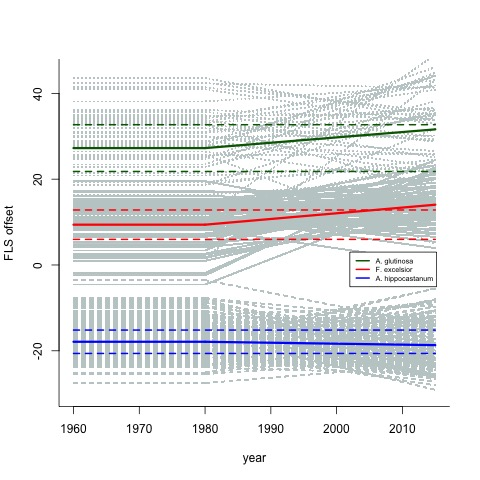
\includegraphics[width=\textwidth]{..//figure/FLS_climate_change.jpeg} 
    \caption{Trends in average FLS offset across Europe for 3 tree species from 1960 to 2015. Dashed lines indicate historic range of FLS variability. All species are increasing their offset, but the rate of change differs between species and and sites}
    \label{fig:Figure 1}
\end{figure}
\begin{figure}
    \centering
    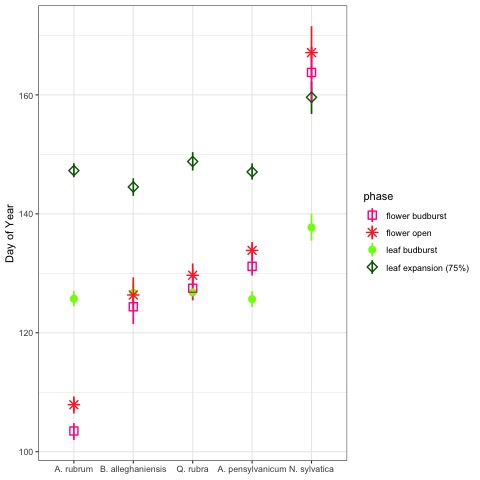
\includegraphics[width=.75\textwidth]{..//figure/HFmeans.jpeg}
    \caption{Average day of phenological events for highlighted woody plant species at Havard Forest in Petersham, MA from 1990-2015}
    \label{fig:Figure 2}
\end{figure}
 \begin{figure}
        \centering
          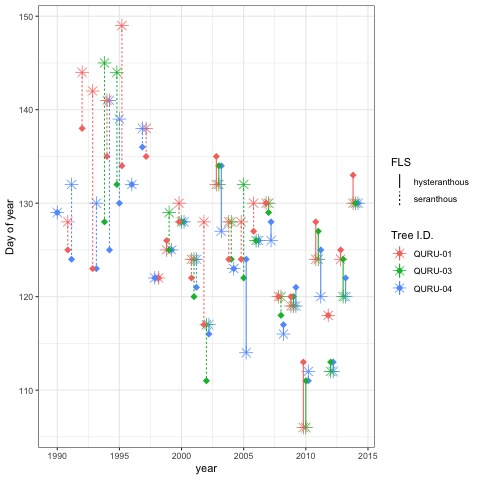
\includegraphics[width=.75\textwidth]{..//figure/HFdissplot.jpeg}
        \caption{FLS variability among years and within a population of \textit{Quercus rubra} at Harvard forest.}
        \label{fig: Figure 3}
    \end{figure}
  
    \begin{figure}
    \centering
    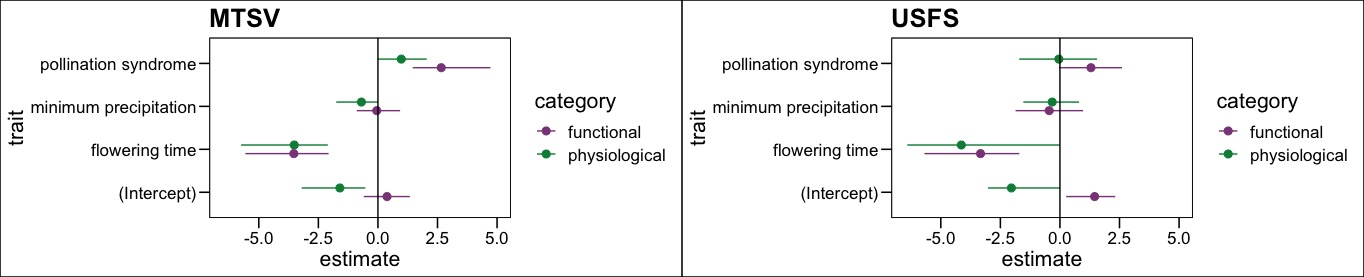
\includegraphics[width=\textwidth]{..//figure/Mtsv_usfs_sidexside.jpeg}
    \caption{Effect size and 95\% bootstrapping intervals estimates}
    \label{fig:Figure 4}
    \end{figure}
    
        \begin{figure}
    \centering
    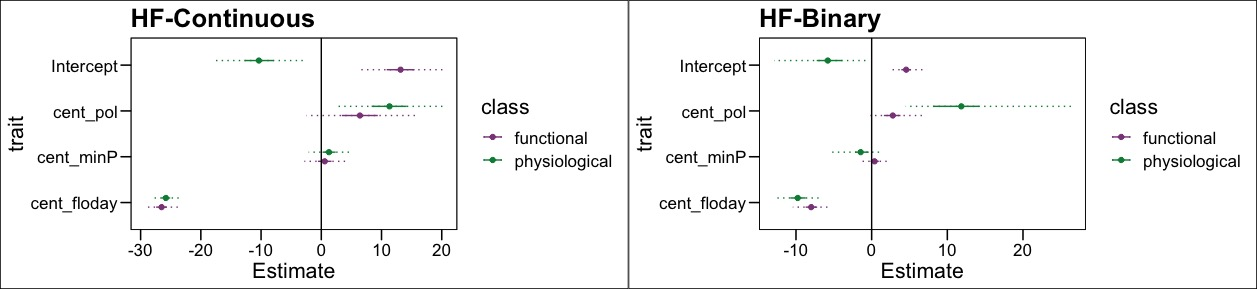
\includegraphics[width=\textwidth]{..//figure/HF_cont_v_bin.jpeg}
    \caption{Harvard forest continuous vs. binary model. Estimates, 50\% and 95\% credible intervals depicted}
    \label{fig:Figure 5}
    \end{figure}



\end{document}
